\chapter{Projets annexes}
{\hypersetup{linkcolor=GREYDARK}\minitoc}
\label{chap:annexes}

\section{Assemblage et annotations du premier génome du hocco à pierre (\textit{Pauxi pauxi})}
\label{annexe:hocco}

Au début de ma thèse, pour le projet de l'étude de la perte convergente du phallus chez les oiseaux (voir Partie \ref{sec:evol-phallus}), nous souhaitions initié le séquençage de plusieurs oiseaux dont la position phylogénétique offre un intérêt particulier pour ce phénotype. Au cours de la première année, nous avons tenté de mettre au point un protocole expérimental d’extraction d’ADN à partir d’échantillons de plumes de poulet ainsi que des plumes de nandou, d’autruche et de casoar fournis par différents zoos (Zoo de Lyon, Zoo de Lille, Parc des Oiseaux de Villars-les-Dombes). Malheureusement, ces extractions n’ont permis d’obtenir que de faibles quantités d’ADN d’une qualité insuffisante pour permettre un séquençage. Cependant, nous avons obtenu des échantillons de sang, contenant de grandes quantités d’ADN, pour le hocco à pierre (\textit{Pauxi pauxi}). Nous avons donc pu générer des données de séquençage pour cette espèce dans le but d'assembler son génome. Parrallèment, le consortium Birds10K publiait de nombreux nouveaux génomes d'oiseaux et un alignement de plus de 360 espèces (sans P.pauxi) \citep{feng_dense_2020}. Nous avons donc abandonner le séquençage des autres oiseaux.\\

Afin d’optimiser l’assemblage de novo nous avons souhaité comparer les résultats de différents assembleurs prometteurs pour nos types de données : IDBA \citep{peng_idba_2010},  DISCOVARdenovo \citep{weisenfeld_comprehensive_2014} et MEGAHIT \citep{li_megahit_2015}. Afin de comparer les résultats nous avons utilisé différentes mesures statistiques données par QUAST \citep{gurevich_quast_2013} comme le nombre de contigs, la taille des contigs, le N50 mais nous avons aussi calculé le nombre de cassures de synténie et la couverture génomique. Nous avons également analysé le nombre de gènes eucaryotes BUSCO, qui sont des orthologues en copie unique connus pour être hautement conservées \citep{simao_busco_2015}, et le nombre de gènes codants pour des protéines du poulet retrouvé dans ces assemblages. Pour l’ensemble des mesures, MEGAHIT a montré les meilleurs résultats. Le génome du hocco nouvellement assemblé possède 39,938 contigs de taille N50 de 42,693 paires de base. Concernant les séquences codantes, 80\% des gènes BUSCO sont retrouvés entièrement et 98,5\% des gènes codant pour des protéines chez le poulet sont retrouvés avec un score d’identité minimum de 60\%. \\

\begin{figure}[h]
    \centering
    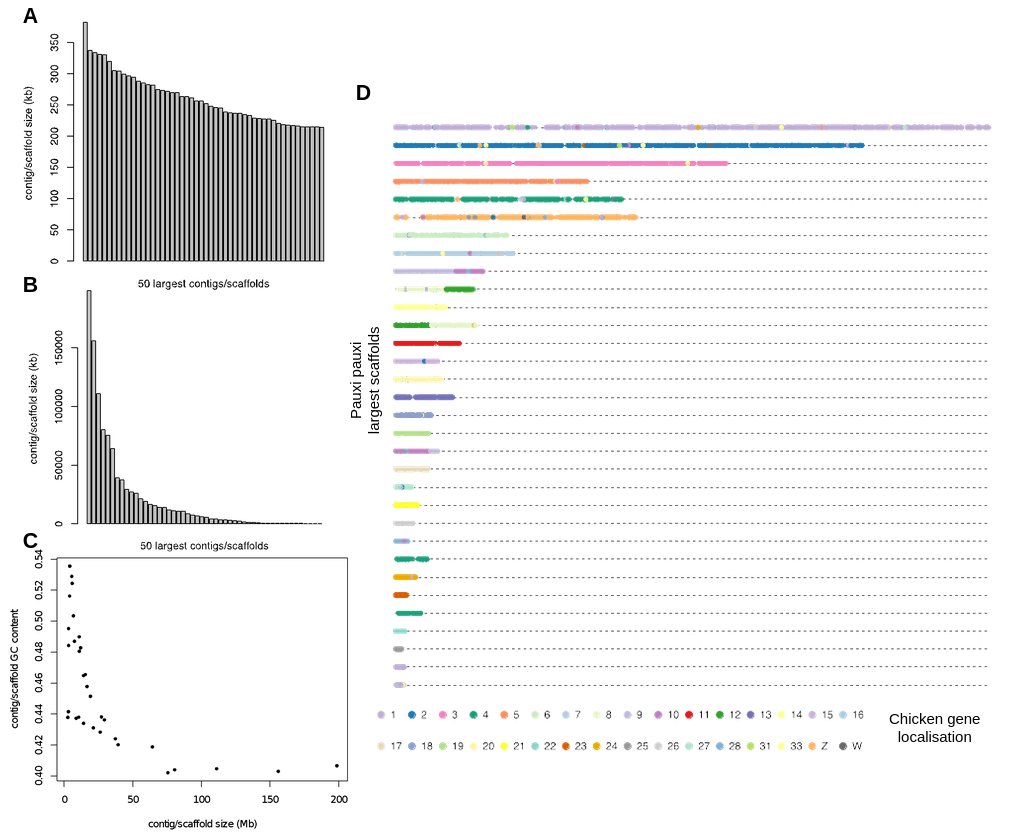
\includegraphics[width=1\textwidth, page=1] {figures/annexes/hocco-fig1.png}
    \caption[Assemblage génomique du hocco.]{
    \textbf{Assemblage génomique du hocco.}. 
    A. Distribution de la taille des 50 plus grands contigs/scaffolds de l'assemblage par MEGAHIT et
    B. après scaffolding par RAGOUT.
    C. Relation entre contenu en GC et la taille des contigs/scaffolds après RAGOUT.
    D. Localisation des gènes orthologues du poulet (\textit{Gallus gallus}) sur les 32 contigs les plus grand du hocco (\textit{Pauxi pauxi}). La couleur des gènes correspond à leur localisation dans le génome du poulet. \\
    }
    \label{fig:hocco-fig1}
\end{figure} 

Nous avons souhaité améliorer l’assemblage génomique du hocco grâce à une approche de scaffolding par homologie avec RAGOUT \citep{kolmogorov_chromosome_2018}. Cet outil permet d'utiliser des génomes de référence d’espèces proches pour réunir des fragments de l’assemblage brouillon par hypothèse de conservation de synténie. Nous avons utilisé les génomes du poulet (\textit{Gallus gallus}), du canard (\textit{Anas platyrhynchos}) et de la pénélope à poitrine rousse (\textit{Penelope pileata}). Ceci a permis d’améliorer significativement l’assemblage génomique passant d’un N50 de 37.5kb à 75 Mb, et d’une longueur de fragment maximum de 381 kb à 198 Mb, s’approchant ainsi d’une résolution chromosomique (Figure \ref{fig:hocco-fig1}.A \& B). Nous avons vérifié la correspondance chromosomique entre ce nouvel assemblage et celui du poulet et du canard en analysant la localisation des gènes homologues (Figure \ref{fig:hocco-fig1}.D). Pour des gènes se trouvant sur le même chromosome dans le génome du poulet ou du canard, leurs homologues dans le génome du hocco sont également majoritairement sur le même fragment génomique. De plus, comme attendu par les conséquences de la recombinaison génique biaisée \citep{galtier_gc-content_2001}, nous observons une corrélation négative entre le contenu en GC et la taille des fragments génomiques reconstruits (Figure \ref{fig:hocco-fig1}.C). Ces analyses nous confortent dans la congruence de cette nouvelle version améliorée de l’assemblage du génome du hocco. \\


\begin{figure}[h]
    \centering
    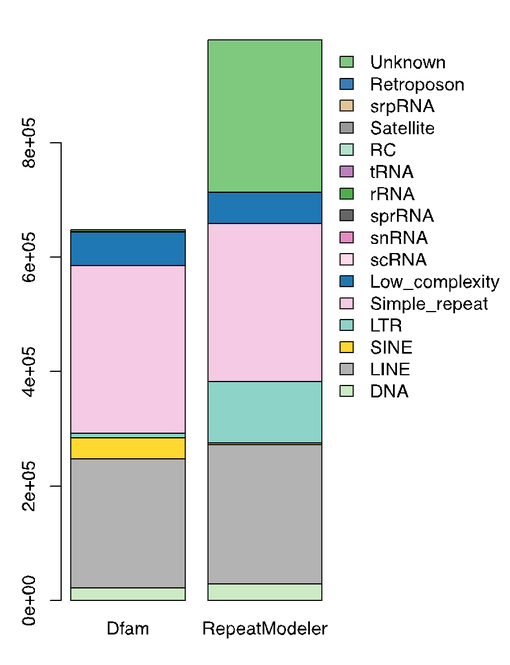
\includegraphics[width=0.5\textwidth, page=1] {figures/annexes/hocco-fig2.png}
    \caption[Annotations du génome du hocco en éléments répétés.]{
    \textbf{Annotations du génome du hocco en éléments répétés.}.  \\
    }
    \label{fig:hocco-fig2}
\end{figure} 

Nous avons également annoté ce nouvel assemblage en éléments répétés, notamment grâce au travail préliminaire de Timothée Kastylevsky, un stagiaire de M2 co-encadré en 2020 et les conseils de Marie Fablet. Une première annotation de novo a été faite avec RepeatModeler \citep{flynn_repeatmodeler2_2020} et une seconde par homologie à l’aide de la base de données Dfam et de RepeatMasker \citep{smit_repeatmasker_2013} (Figure \ref{fig:hocco-fig2}. L’annotation en gènes a été faite avec GeMoMa \citep{kollmar_gemoma_2019} et à l’aide de protéines de référence annotées par Ensembl à partir de plusieurs espèces d’oiseaux, de reptiles et de mammifères \citep{cunningham_ensembl_2019}. \\

Nous avons ensuite utilisé Progressive Cactus \citep{armstrong_progressive_2020} pour aligner ce génome avec d’autres oiseaux en l’intégrant dans l’alignement de génomes complets des plus de 360 oiseaux \citep{feng_dense_2020}. Cette étape a été essentielle pour utiliser le génome du hocco dans l’analyse de la convergence évolutive du paysage cis-régulateur en lien avec la présence du phallus présentée en Partie \ref{IPLOSS}. \\

Finalement, cet oiseau possède une excroissance osseuse sur le crâne similaire à plusieurs lignées d’oiseaux \citep{mayr_survey_2018}. Nous avons voulu tester si nous pouvions détecter un lien entre la convergence de ce phénotype et les séquences codantes d'une sélection de 28 oiseaux dont 8 possède une telle excroissance (Figure \ref{fig:hocco-fig3}.A). Nous avons dans un premier temps reconstruit les familles des gènes orthologues un-à-un à l’aide d’OrthoFinder \citep{emms_orthofinder_2019}. Nous avons ensuite effectué un alignement des séquences protéiques avec PRANK \citep{loytynoja_phylogeny-aware_2014}. A l'aide de PELICAN, un outil non publié développé par des collègues du LBBE, nous avons calculer pour chaque gène un score d'association entre la convergence du profil d’acides aminés et la présence/absence d'une excroissance osseuse (Figure \ref{fig:hocco-fig3}.B). Pour les gènes significativement associé à la présence de ce phénotype, nous avons observer un enrichissement pour des fonctions connus pour être associés à des malformations du crâne chez la souris. \\

\begin{figure}[h]
    \centering
    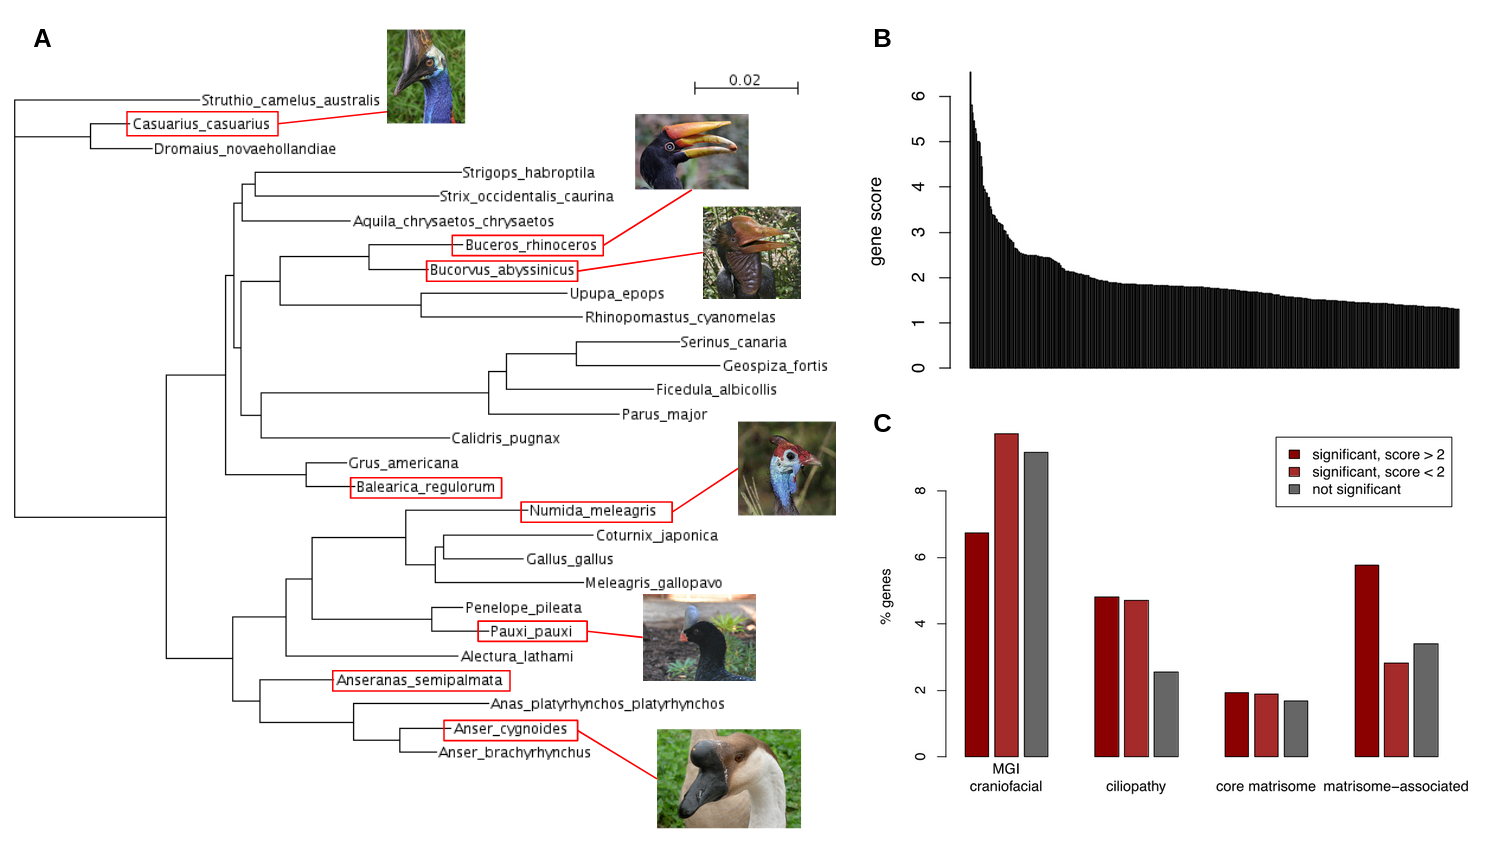
\includegraphics[width=1.2\textwidth, page=1] {figures/annexes/hocco-fig3.png}
    \caption[Association entre l'évolution des séquences codantes et la présence d'une excroissance osseuse.]{
    \textbf{Association entre l'évolution des séquences codantes et la présence d'une excroissance osseuse.}
    A. Phylogénie des 28 oiseaux considérés. Les espèces encadrés en rouge présentent une convergence d'une excroissance osseuse.
    B. Distribution des scores d'associations entre la convergence du profil d’acides aminés et la présence/absence du phénotype.
    C. Enrichissement des gènes qui présentent une convergence significative du profil d'acides aminés selon la présence d'une excroissance pour des fonctions connus pour être associés à des malformations du crâne chez la souris. \\
    }
    \label{fig:hocco-fig3}
\end{figure} 

\newpage
\section{Modélisation du réseau de régulation du gène ACE2 impliqué dans l’infection et la réponse au Sars-Cov-2}
\label{annexe:ACE2}

Durant le premier confinement lié à la pandémie actuelle, plusieurs initiatives de recherche en lien avec le virus ont émergé au LBBE. L’une d’entre elles, portée par Etienne Rajon en collaboration avec le pôle Santé du LBBE ainsi que le laboratoire BF2i de l'INSA de Lyon, nous a été proposée à Anamaria et moi-même. L'objectif de celle-ci est de mieux comprendre la dynamique de régulation du gène ACE2, qui est impliqué dans la physiologie du Covid-19. Ce gène produit une protéine trans-membranaire présente à la surface de nombreuses cellules, notamment dans les voies respiratoires chez l’humain. Cette protéine est un des récepteurs principaux du virus SARS-CoV-2 et permet son entrée dans les cellules de l’hôte \citep{hoffmann_sars-cov-2_2020}. Le patron d’expression d’ACE2 est un élément clé dans l’infection car sa surexpression pourrait alors augmenter les opportunités d’entrée du virus. D’un autre côté, l’augmentation de la charge virale dans l’organisme de l’hôte entraîne l’occupation des protéines d’ACE2 effectives et perturbe alors leur rôle fonctionnel dans l’organisme, qui pourrait notamment assurer une protection aux lésions pulmonaires \citep{imai_angiotensin-converting_2005}. Une faible expression basale du gène pourrait alors avoir des conséquences importantes sur l’organisme suite à une infection et participerait à aggraver la sévérité des symptômes. La relation entre l’expression d’ACE2, l’infection du SARS-CoV-2 et la sévérité du Covid-19 est alors complexe. L’objectif de ce projet est de tenter de modéliser l’expression d’ACE2 pour prédire son expression dans les cellules ciblées par le virus et la dépendance de son patron d’expression selon le génotype du patient (Figure \ref{fig:ace2}.A). \\

\begin{figure}[h]
    \centering
    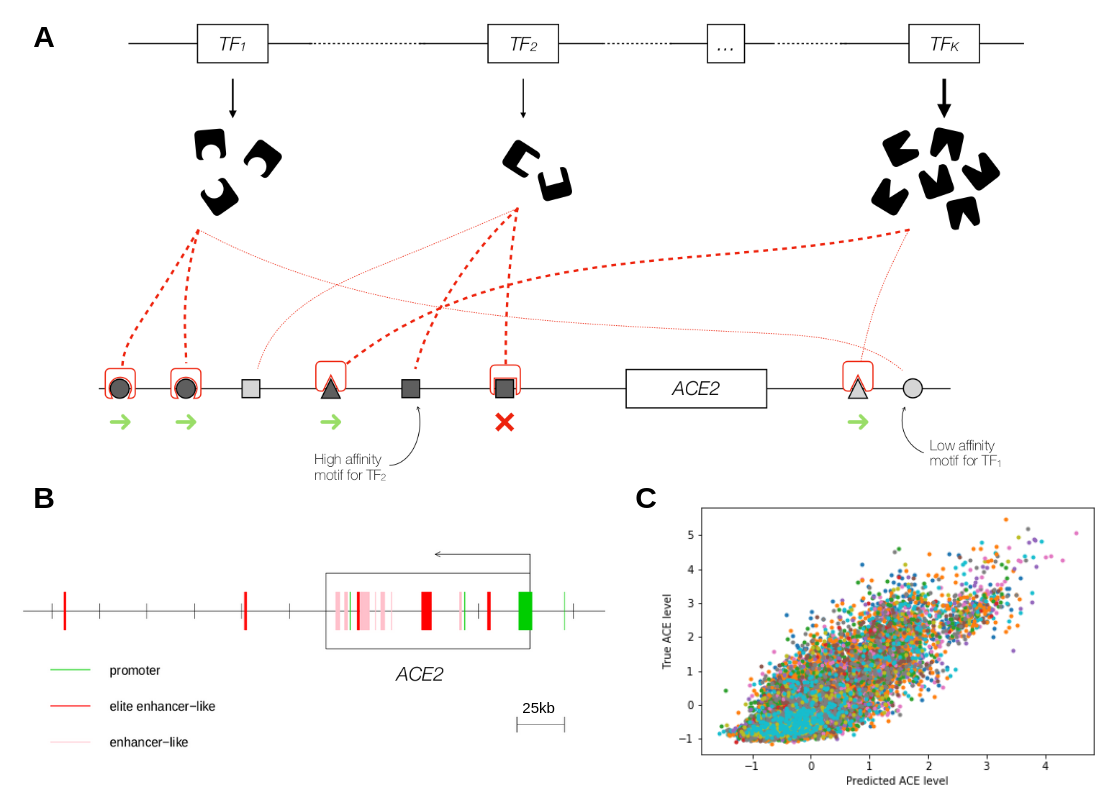
\includegraphics[width=1\textwidth, page=1] {figures/annexes/ace2-fig1.png}
    \caption[Modélisation du réseau de régulation du gène ACE2.]{
    \textbf{Modélisation du réseau de régulation du gène ACE2}
    A. Description du réseau de régulation d'ACE2 considéré dans le modèle. L'expression des gènes codants pour des facteurs de transcription (TFs) est spécifique de l'échantillon considéré et permet de produire une quantité de protéine à une concentration mesurable. Ces protéines peuvent se fixer sur des séquences \textit{cis}-régulatrices selon une probabilité qui dépend de l'affinité du motif aux sites de fixation. La fixation des TFs sur une séquence \textit{cis}-régulatrice peut activer/amplifier (flèche verte) ou réprimer (croix rouge) la transcription d'ACE2.
    B. Localisation des séquences\textit{cis}-régulatrices de l'expression d'ACE2 d'après GenHancer \citep{fishilevich_genehancer_2017}.
    C. Prédiction du niveau d'expression d'ACE2 selon les niveaux d'expression d'une sélection de TFs. \\
    }
    \label{fig:ace2}
\end{figure} 

Ma contribution dans ce projet a été d’apporter des éléments de réponse quant aux mécanismes qui sous-tendent la régulation de l’expression d’ACE2. Mon premier rôle a été d’identifier des séquences \textit{cis-}régulatrices potentielles d’ACE2. Pour ce faire, j’ai utilisé les données de PCHiC utilisées dans mon premier axe ainsi que plusieurs sources de données publiques telles que les inférences de régulation de FOCS \citep{hait_focs_2018}, les informations génomiques du voisinage direct du gène, ainsi que la base de données de GenHancer qui intègre des données de diverses sources (ChIP-seq, DHS-seq, eRNA et HiC) \citep{fishilevich_genehancer_2017}. Ces différentes approches complémentaires m’ont permis d’obtenir une liste de 17 séquences candidates avec différents degrés de confiance (Figure \ref{fig:ace2}.B).J’ai apporté un élément supplémentaire au modèle qu’est l’accessibilité de la chromatine via des données publiques récentes de DHS-seq dans de nombreux échantillons humains \citep{meuleman_index_2020}. En recoupant ces données avec les séquences régulatrices candidates d’ACE2, nous pouvons inférer lesquelles sont accessibles et donc potentiellement actives en fonction des tissus. Mariana Ferrarini et Sergio Peignier au BF2i, ont quant à eux analysé la corrélation de l'expression d'ACE2 et des facteurs de transcription grâce à des données publiques de transcriptomiques (RNAseq) issus de plusieurs tissus humains. L'objectif était de pouvoir prédire le niveau d'expression d'ACE2 dans des tissus à partir de l'expression d'une sélection des facteurs de transcription les plus explicatifs (Figure \ref{fig:ace2}.C). \\

En raison de résultats peu concluants rapidement et surtout du manque d'implication sur le long terme des différents participants, ce projet n’a finalement pas abouti et est actuellement au point mort.

\newpage
\section{Conséquence de la perte de PRDM9 sur l’évolution des îlots de régulation CpG chez les Canidae}
\label{annexe:canidae}

J'aurais été déçu de faire une thèse sans collaborer scientifiquement avec mes amis doctorants au LBBE. Alors quand Julien Joseph nous a réuni avec Théo Tricou, Djivan Prentout, Thibault Latrille et Florian Benitière pour des conseils et “expertises” issus de nos thèses respectives pour un projet, je n’ai pas pu m’empêcher de m’investir. \\

Ce projet vise à caractériser les conséquences de la perte de PRDM9, gène responsable du positionnement des points chauds de recombinaison pendant la méiose, sur la composition nucléotidique des génomes des Canidae. L’hypothèse est que la perte de PRDM9 chez les Canidae a entraîné une stabilisation de la localisation des points chauds de recombinaison \citep{baudat_prdm9_2010}. En raison de la conversion génique biaisée (gBGC), ces points chauds stabilisés subiraient alors une accumulation de substitutions vers les nucléotides G et C \citep{galtier_gc-content_2001}. Nous nous intéressons plus particulièrement aux dinucléotides CpG, qui, regroupés en îlots aux abords des promoteurs et selon leur méthylation, peuvent jouer un rôle important dans la régulation de l’expression des gènes \citep{deaton_cpg_2011}. Nous cherchons à quantifier les gains/pertes d’îlots CpGs (CGIs) le long de la phylogénie des carnivores en comparant les Canidae aux Felidae et Phocidae, groupes frères possédant encore un PRDM9 fonctionnel et donc des points chauds instables. Une deuxième étape sera ensuite d’estimer les relations entre l’évolution de ces séquences et l’évolution de l’expression des gènes. \\

En plus des discussions pour définir le projet, mon premier rôle a été de générer un alignement de 19 génomes complets issus d'espèces de carnivores à l’aide de Progressive Cactus \citep{armstrong_progressive_2020} et de créer des chaînes LiftOver \citep{kent_human_2012} entre génomes pour accéder facilement aux relations d’homologies des CGIs. Grâce au travail de Théo Tricou et après l'annotation en gènes de certains génomes, nous disposons également d’une phylogénie basée sur les séquences codantes de ces espèces (Figure \ref{fig:canidae}.A). Récemment, Djivan Prentout et Julien Joseph ont déterminé les coordonnées des îlots CpGs de chaque espèce. A partir des alignements de génome, j'ai ainsi pu extraire les CGIs homologues et déterminés leur conservation ou leur perte entre les espèces (Figure \ref{fig:canidae}.B). Finalement, Florian Bénitière a récupéré et traité des données d’expression des gènes dans plusieurs tissus chez 13 des 19 espèces de carnivores. La suite pour mes collègues sera alors de faire tourner un modèle bayésien de gain/perte pour calculer les taux d’évolution des CGIs le long de la phylogénie. Grâce aux différentes méthodes que j'ai pu mettre en place au cours de ma thèse, nous allons finalement associer les CGIs aux gènes qui se situent au voisinage ou pourquoi pas étant en contact physique d'après des données de conformation de la chromatine (Hi-C). Nous évaluerons finalement les relations entre les gains/pertes de CGI et l’activité transcriptionnelle des gènes avec des méthodes comparatives phylogénétiques de type PGLS \citep{adams_phylogenetic_2019, rohlf_comparative_2001}.

\begin{figure}[h]
    \centering
    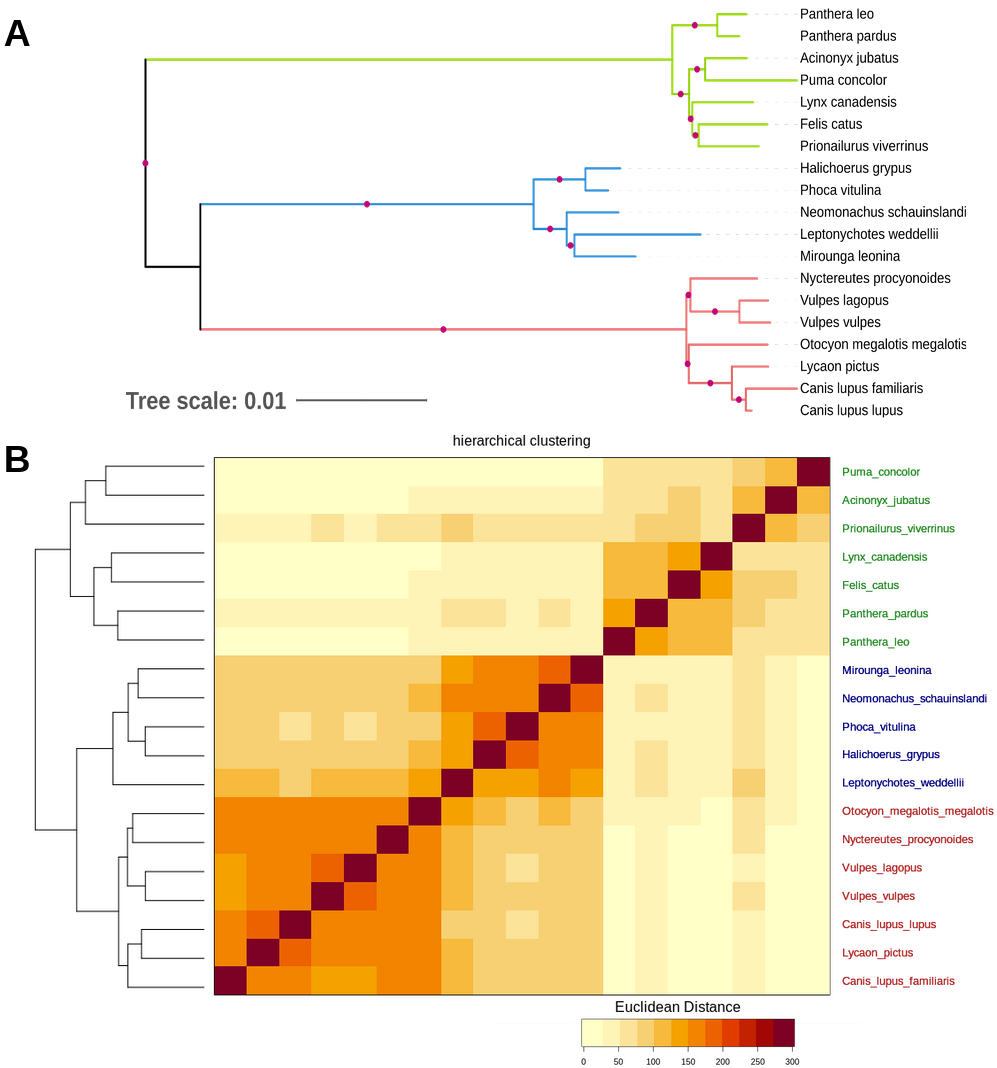
\includegraphics[width=1\textwidth, page=1] {figures/annexes/Canidae-fig1.png}
    \caption[Relation phylogénétique et conservation des îlots CpGs chez les Carnivores.]{
    \textbf{Relation phylogénétique et conservation des îlots CpGs chez les Carnivores.}
    A. Arbre phylogénétique des 19 espèces de Carnivores étudiées obtenus à partir des séquences codantes de X gènes orthologues.
    B. Regroupement hiérarchique des espèces à partir de la conservation (présence/absence) de l'ensemble des 249,008 îlots CpGs détectés dans toutes les espèces.\\
    }
    \label{fig:canidae}
\end{figure} 


\chapter{Annexes}
{\hypersetup{linkcolor=GREYDARK}\minitoc}
\label{chap:annexes}

\section{Article 2 - Figures complémentaires}
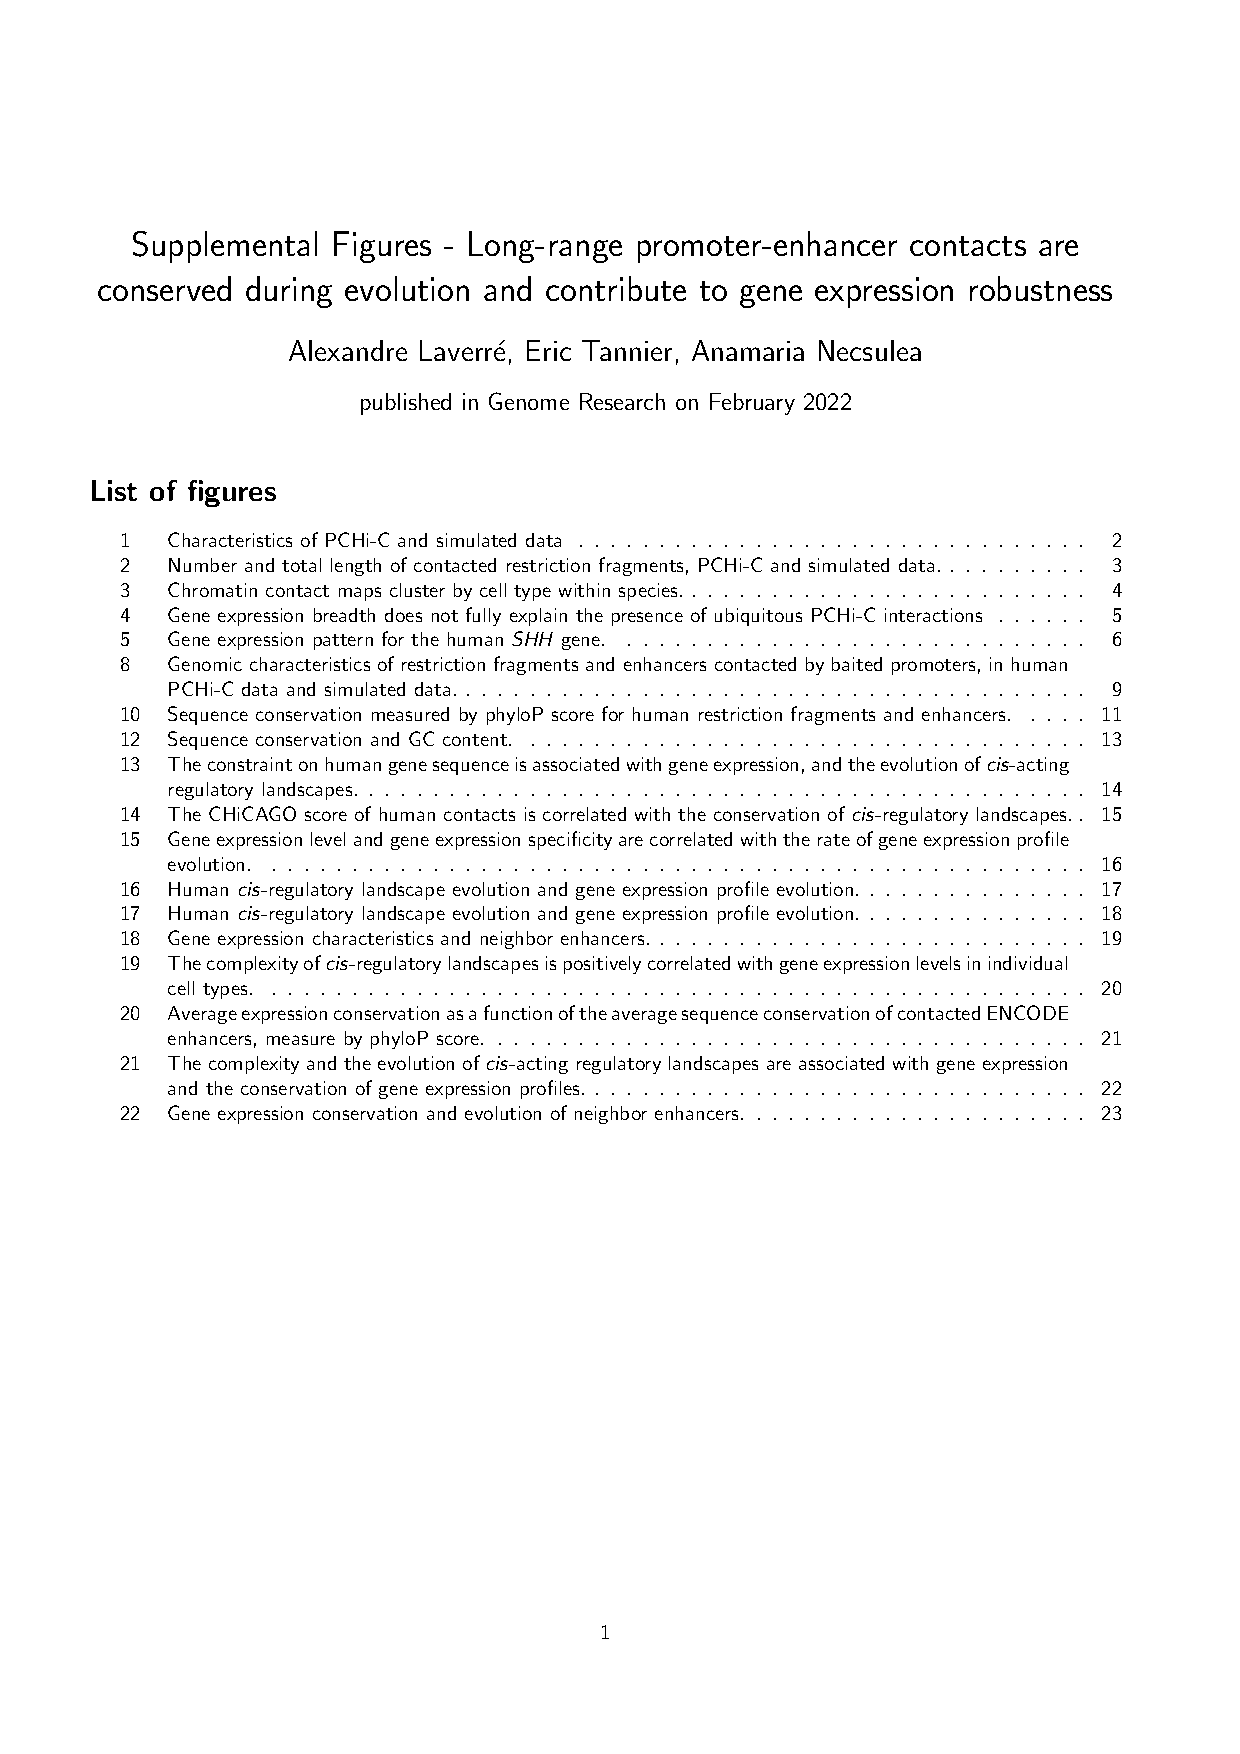
\includepdf[pages=-]{annexes/Supp_Figures_Laverre2022.pdf}

\section{Article 2 - Texte et figures supplémentaires}
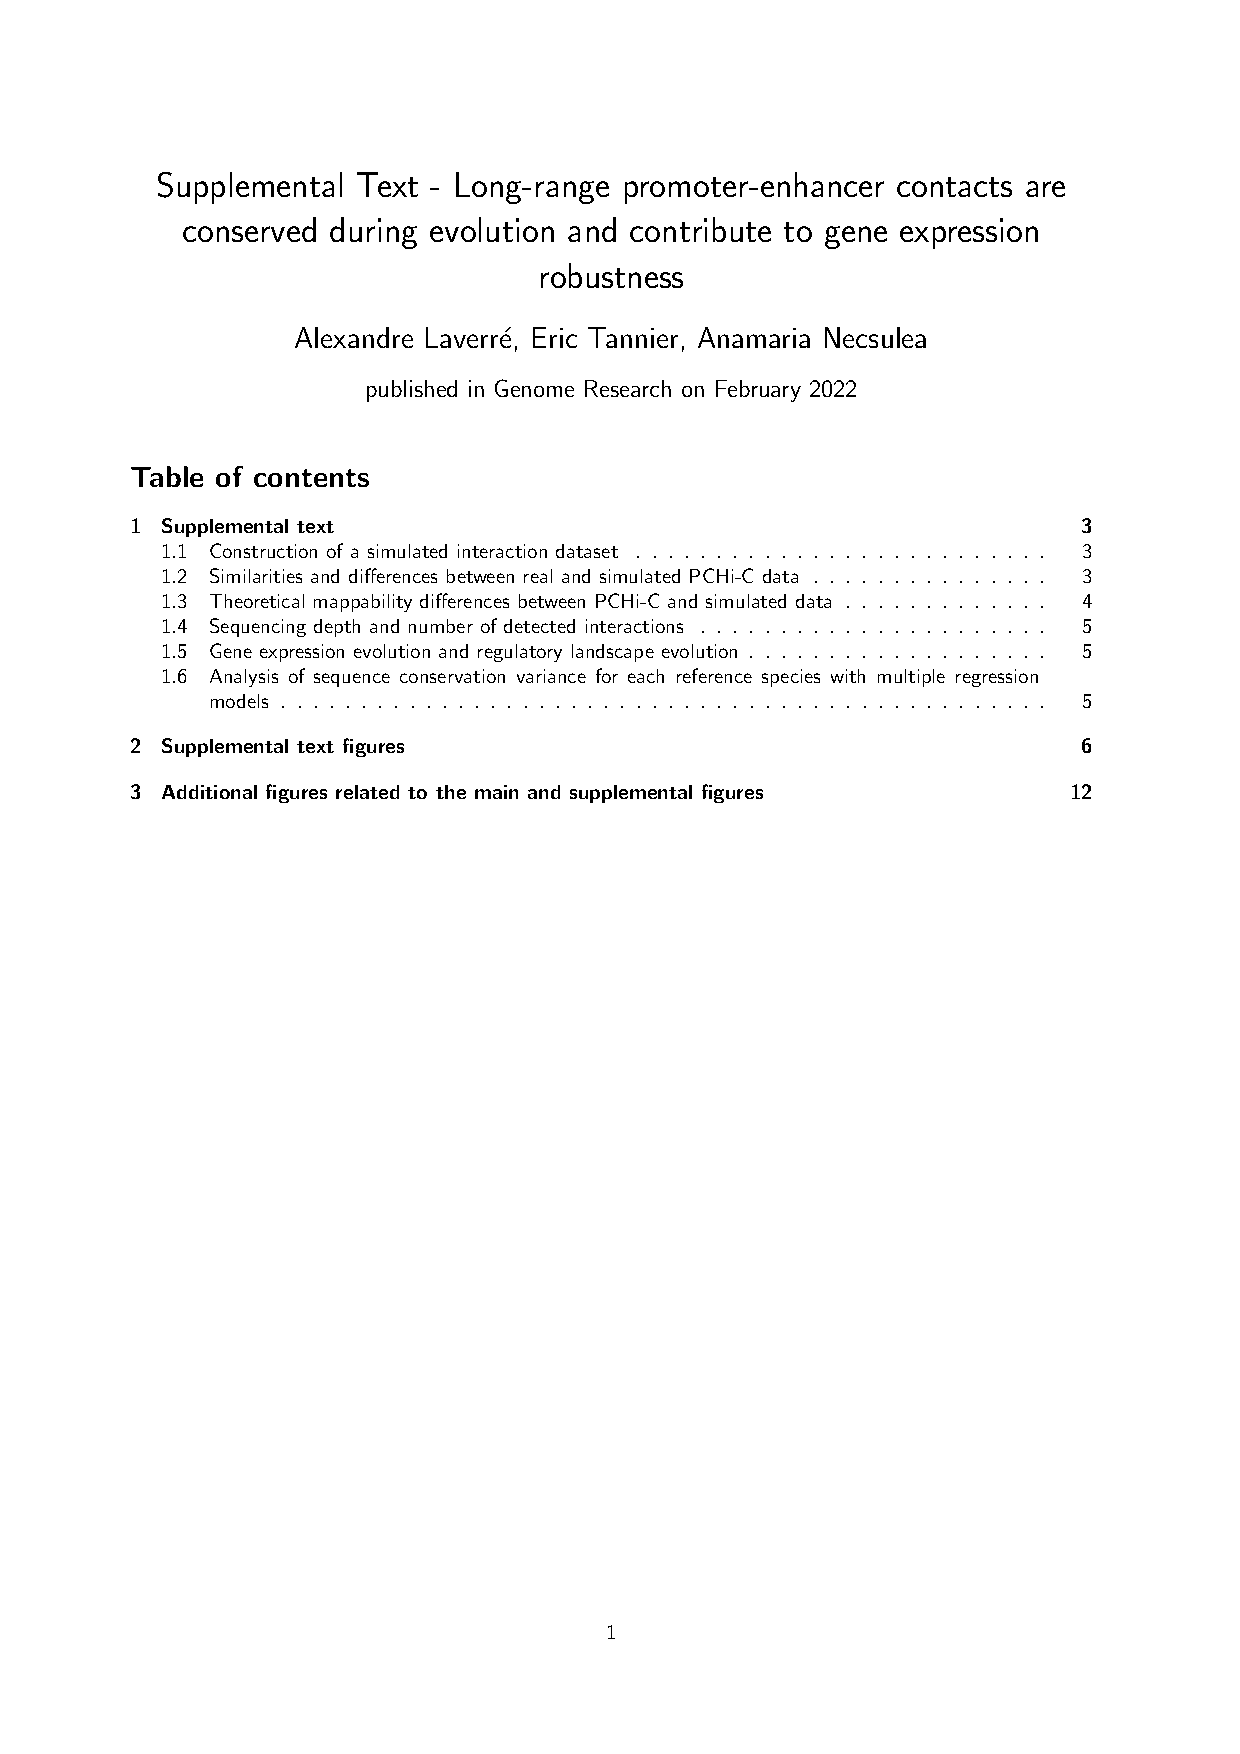
\includepdf[pages=-]{annexes/Supp_Text_Laverre2022.pdf}

